\section{Terrain Classifier Creation (2 pages)}

We will create multiple methods and evaluate them on their ability to predict the
safety mask of the landing sites in the synthetic data sets.
We will focus first on using U-nets to map from the input LIDAR or RGBD image
to the output mask, as they have been proven to be good classifiers in many different scenarios,
from terrain analysis, to tissue analysis, to road identification, etc.
We anticipate that the main challenge in this domain will not be
to train the networks, but rather to keep them small enough
so that they can execute quickly on embedded hardware.
Nevertheless, we will start by focusing strictly on maximizing the ability of the networks
to accurately predict the safety masks.

\subsection{Pre-Processing}

An unavoidable step in this process is preprocessing the input data.
In the case of RGBD images, we should rectify input to remove sensor distortion.
This is helpful for understanding what the data truly represents,
and also removes sensor biases, so that the terrain analysis methods do not overfit to data from a particular sensor.
We will also transform input according to IMU tags in order to properly identify slants.
One option for pre-processing in the case of LIDAR point clouds is to convert them to depth images.
In either case, the input must be normalized with respect to sensor calibration data -
sensors tend to auto-adjust their scales in order to clarify differences in values at each point.
This occurs when RGB cameras auto-adjust brightness in order to make a clearer picture,
and also when an RGBD camera detects the average range of detected depths, and adjusts its format accordingly.
Finally, downsizing input images and point clouds is a common method of computational speedup
that will most likely be necessary, given that the target hardware platforms are limited, embedded boards.

\subsection{Topological Analysis}

The most important aspect of a safe landing site is its topology.
We want to identify regions of the pre-processed input images that are sufficiently flat and large.
Signal processing methods, such as analysis of the image's gradient, and even edge detection algorithms (e.g.~Canny, etc.)
can be used to detect contiguous flat regions.
Deep learning methods such as pooling and 2D convolutions can accomplish similar tasks.
The most relevant data channel in an RGBD image for topological analysis is the depth channel,
but other channels could still offer useful information.
While it is possible to ``hand-make'' a solution for finding a landing region that is topologically viable,
it may also be useful to train deep learning methods to do this task.
They will likely have inherent biases that are different from the hand-made solutions,
which will give a wider view of the solution space in the worst case,
and which will yield better results in the best case.
Moreover, a deep learning method will be more suited to use the embedded TPU and GPU on the target companion boards,
and therefore may run faster.

\subsection{Semantic Segmentation}



We will use a U-net or residual u-net, or conventional CNN for basic semantic segmentation of the pre-processed input images.


As an example of how this will work, we take an example from my project in RU's Deep Learning
course, wherein my group member and I used a Residual U-net to classify defects
in manufactured steel.
More than 17,000 images were labeled by hand, according to which of 4 defects they contained.
Figure~\ref{figure:example_steel_prediction} shows an example of the input data from this project,
where the yellow and blue outlines show the locations of different types of defect areas.

This particular project was very time-limited, so the network trained for only 4 epochs,
but was able to achieve about 50\% prediction accuracy in that time,
and its output for an example image can be seen in Figure~\ref{figure:example_steel_prediction}.
This project also gave some insight into accuracy metrics that can help bias the output
for/against false positives/negatives.
For example, in the case of the steel defect recognition, we used a Tversky metric to
reduce the amount of false negative defect classifications because a second step of the
process is for a human to manually examine the defect-classified steel before discarding it.
In this context it is better to make the network more ``cautious,'' in the hopes that
alerting the human to some false defects will mean that the network never incorrectly approves
defected steel for sale.
Conversely, in the case of autonomous drones,
we would like the networks to be conservative in their identification of safe landing sites,
so that they never direct the drone to land in unsafe landing sites, even though they may reject
some landing sites that are actually safe.
This is purely to give an intuition of the form of the problem we will use the classifiers to solve.

\begin{figure}
    \centering
    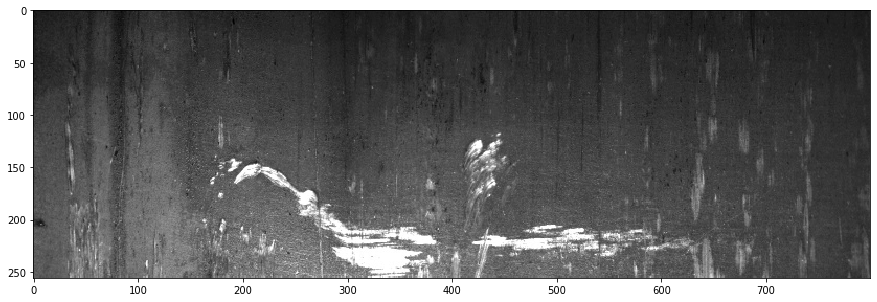
\includegraphics[width=\textwidth]{images/original_image.png}
    \subfloat[Defect 1 Mask]{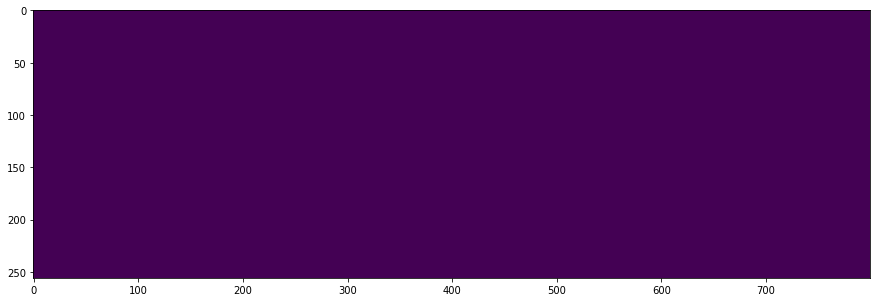
\includegraphics[width = 0.5\textwidth]{images/true_def0.png}}
    \subfloat[Defect 1 Prediction]{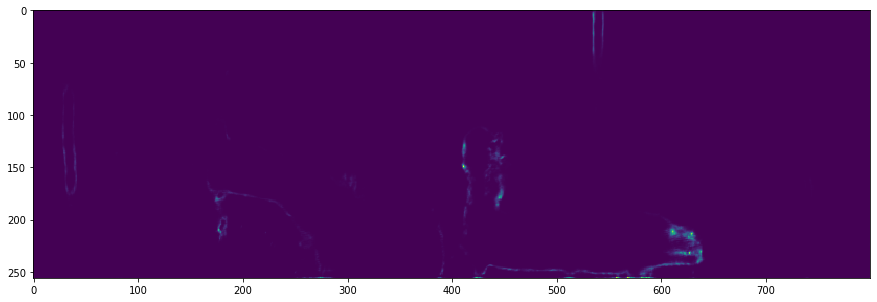
\includegraphics[width = 0.5\textwidth]{images/pred_def0.png}}\\
    \subfloat[Defect 2 Mask]{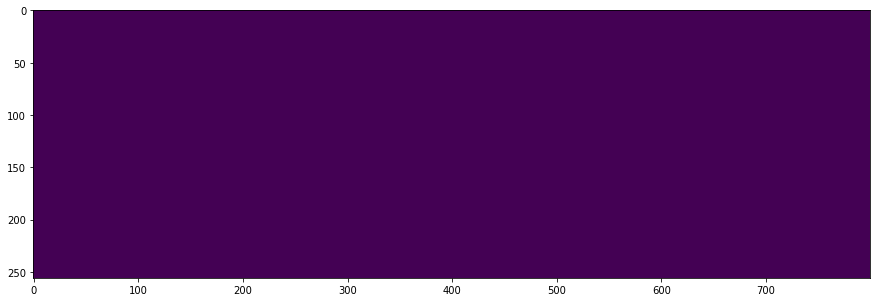
\includegraphics[width = 0.5\textwidth]{images/true_def1.png}}
    \subfloat[Defect 2 Prediction]{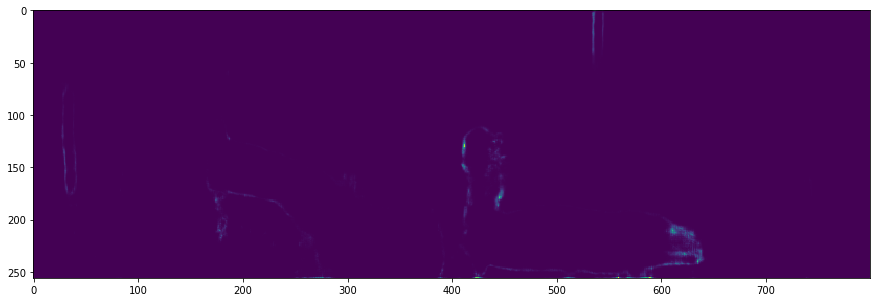
\includegraphics[width = 0.5\textwidth]{images/pred_def1.png}}\\
    \subfloat[Defect 3 Mask]{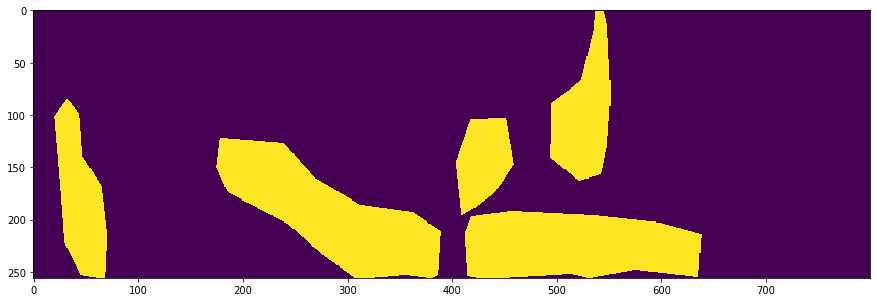
\includegraphics[width = 0.5\textwidth]{images/true_def2.png}}
    \subfloat[Defect 3 Prediction]{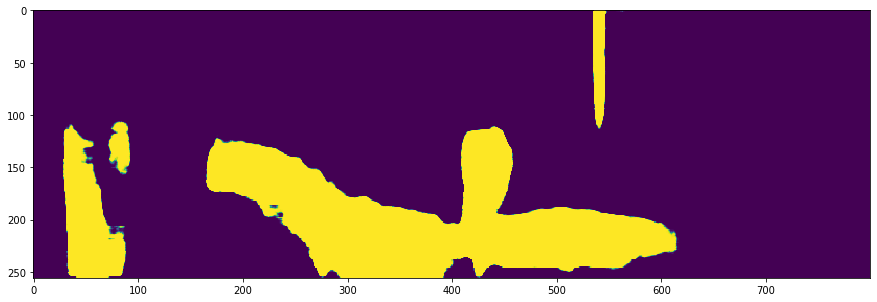
\includegraphics[width = 0.5\textwidth]{images/pred_def2.png}}\\
    \subfloat[Defect 4 Mask]{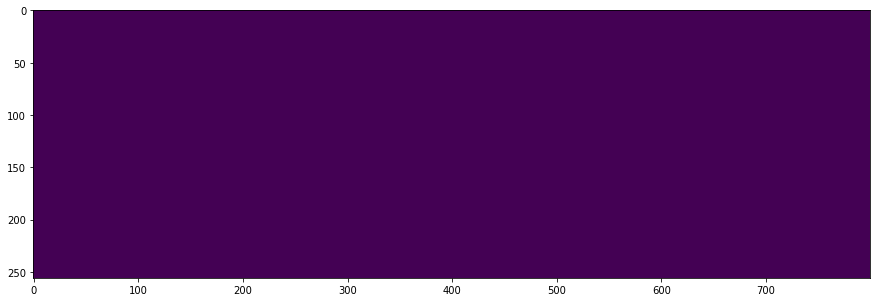
\includegraphics[width = 0.5\textwidth]{images/true_def3.png}}
    \subfloat[Defect 4 Prediction]{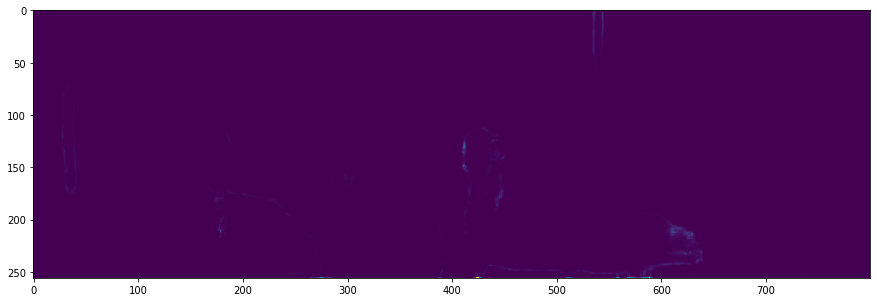
\includegraphics[width = 0.5\textwidth]{images/pred_def3.png}}
    \caption{A visualization of the network's performance in predicting defects.}
    \label{figure:example_steel_prediction}
\end{figure}